% =============================================================================
%  A Radix-4 Booth Multiplier in Structural VHDL
%  Build:  pdflatex report.tex   (run twice, for the table of contents)
% =============================================================================
\documentclass[11pt,a4paper]{article}

\usepackage[T1]{fontenc}
\usepackage[utf8]{inputenc}
\usepackage{lmodern}
\usepackage[margin=2.4cm]{geometry}
\usepackage{amsmath,amssymb}
\usepackage{booktabs}
\usepackage{graphicx}
\usepackage{xcolor}
\usepackage{microtype}
\usepackage{listings}
\usepackage{caption}
\usepackage[section]{placeins}
\usepackage{etoolbox}
\usepackage[hidelinks]{hyperref}

% Keep every float inside the (sub)section that introduces it: placeins gives
% the barrier at \section, this extends it to \subsection.
\preto\subsection{\par\FloatBarrier}
% and prefer here/top, so a float lands where it is declared
\makeatletter
\renewcommand{\fps@figure}{!ht}
\renewcommand{\fps@table}{!ht}
\makeatother
\setcounter{topnumber}{3}
\setcounter{totalnumber}{4}
\renewcommand{\topfraction}{0.9}
\renewcommand{\textfraction}{0.08}
\renewcommand{\floatpagefraction}{0.75}

\definecolor{codebg}{HTML}{F7F6F2}
\definecolor{rule}{HTML}{B4B2A9}
\definecolor{accent}{HTML}{185FA5}
\definecolor{soft}{HTML}{5F5E5A}

\lstset{
  basicstyle=\ttfamily\footnotesize,
  backgroundcolor=\color{codebg},
  frame=single, rulecolor=\color{rule}, framesep=5pt,
  breaklines=true, showstringspaces=false,
  columns=fullflexible, keepspaces=true, xleftmargin=0pt,
  commentstyle=\color{soft}\itshape,
}
\lstdefinestyle{vhdl}{language=VHDL,
  morekeywords={architecture,entity,generate,downto,natural,variable,signal,configuration,constant}}

\captionsetup{font=small, labelfont={bf,color=accent}}

% provenance tag: ties a measured number to the synthesis report it was read from
\newcommand{\src}[1]{\,{\footnotesize\color{accent}[#1]}}

\title{\textbf{A Radix-4 Booth Multiplier in Structural VHDL}\\[4pt]
       \large Architecture, optimization and synthesis at 32 bits in Nangate 45\,nm}
\author{Erfan Taheri}
\date{Nangate 45\,nm Open Cell Library \quad$\cdot$\quad Synopsys Design Compiler \quad$\cdot$\quad ModelSim}

\begin{document}
\maketitle

\begin{abstract}
\noindent
This report presents the design and optimization of a generic signed radix-4
Booth multiplier described in structural VHDL, together with the synthesis
results obtained for the $32\times32$-bit instance using Synopsys Design
Compiler and the Nangate 45\,nm library. Three reduction strategies are
implemented behind a single entity interface: a behavioural summation of the
partial products, a Wallace carry-save adder tree, and a Dadda tree. Three
architectural optimizations are then applied in sequence: elimination of the
partial-product sign extension in favour of a constant correction vector,
replacement of the Wallace tree by a generic Dadda schedule computed at
elaboration time, and fusion of the Booth selection and negation steps into a
single compound gate per bit. Each optimization is derived analytically,
implemented as an alternative VHDL architecture, verified in simulation and
measured over a sweep of clock constraints. A multiplier inferred by the
synthesis tool from a plain \texttt{A * B} statement is synthesised under
identical conditions and used as an absolute reference point.

The final design reaches a minimum achieved period of
\textbf{1.76\,ns}\src{R4} against \textbf{1.63\,ns}\src{R6} for the inferred
reference, and a minimum area of \textbf{5029\,um$^2$}\src{R4} against
\textbf{4441\,um$^2$}\src{R6}. Relative to the unoptimized Wallace
baseline, the three optimizations together recover \textbf{69\%} of the area
difference between the structural design and the inferred reference.
Every measured quantity in this report carries a tag such as \src{R4}
identifying the synthesis report it was read from; the key is given in
Appendix~\ref{app:prov}.
\end{abstract}

\tableofcontents
\clearpage

% =====================================================================
\section{Introduction}

The objective of this work is a hand-built signed multiplier that comes as close
as possible to the multiplier Design Compiler infers from a plain \texttt{A * B}
statement, and a quantitative account of where the remaining difference lies.
The inferred design is a mature, tuned implementation; treating it as a fixed
target turns every architectural decision into a measurable one.

The design is a radix-4 Booth multiplier written in structural VHDL, generic in
the operand width $N$ and instantiated at $N=32$, signed, with the product taken
modulo $2^{2N}$. Three architectural optimizations are applied in sequence ---
elimination of the partial-product sign extension, a Dadda reduction schedule in
place of a Wallace tree, and fusion of the Booth selection and negation steps.
Each is derived analytically, implemented as an alternative VHDL architecture,
verified against a reference model, and measured over a sweep of clock
constraints.

Three constraints govern the implementation throughout:

\begin{itemize}\itemsep2pt
\item \textbf{Single source tree.} Every variant is an alternative
      \texttt{architecture} of an existing entity, selected by a VHDL
      \texttt{configuration}. No file is duplicated, so a variant differs from
      its predecessor only in the component it binds, and the measured
      difference is attributable to that component alone.
\item \textbf{Absolute reference.} The inferred \texttt{A * B} design is
      synthesised with the same script, constraints and library, so results are
      absolute rather than relative to an arbitrary baseline.
\item \textbf{Verification precedes measurement.} A variant is synthesised only
      after it passes the self-checking testbench exhaustively at $N=8$. Area
      and timing reports do not distinguish a correct design from an incomplete
      one, so functional equivalence is established first.
\end{itemize}

Section~\ref{sec:arch} describes the architecture and establishes the
modular-arithmetic framework on which the first optimization depends.
Sections~\ref{sec:opt1}--\ref{sec:opt3} derive, implement and measure the three
optimizations. Section~\ref{sec:verif} describes the verification strategy,
Section~\ref{sec:method} the synthesis methodology, and
Section~\ref{sec:results} the measured results. Source organisation and the
configuration mechanism are documented in Appendix~\ref{app:code}.

% =====================================================================
\section{Architecture}
\label{sec:arch}

The datapath is shown in Figure~\ref{fig:schem}: Booth encoders drive one
row generator each, a corrector supplies one additional row, a reduction tree
compresses the $N/2+1$ rows to two, and a carry-propagate adder produces the
$2N$-bit product.

\begin{figure}[!ht]
\centering
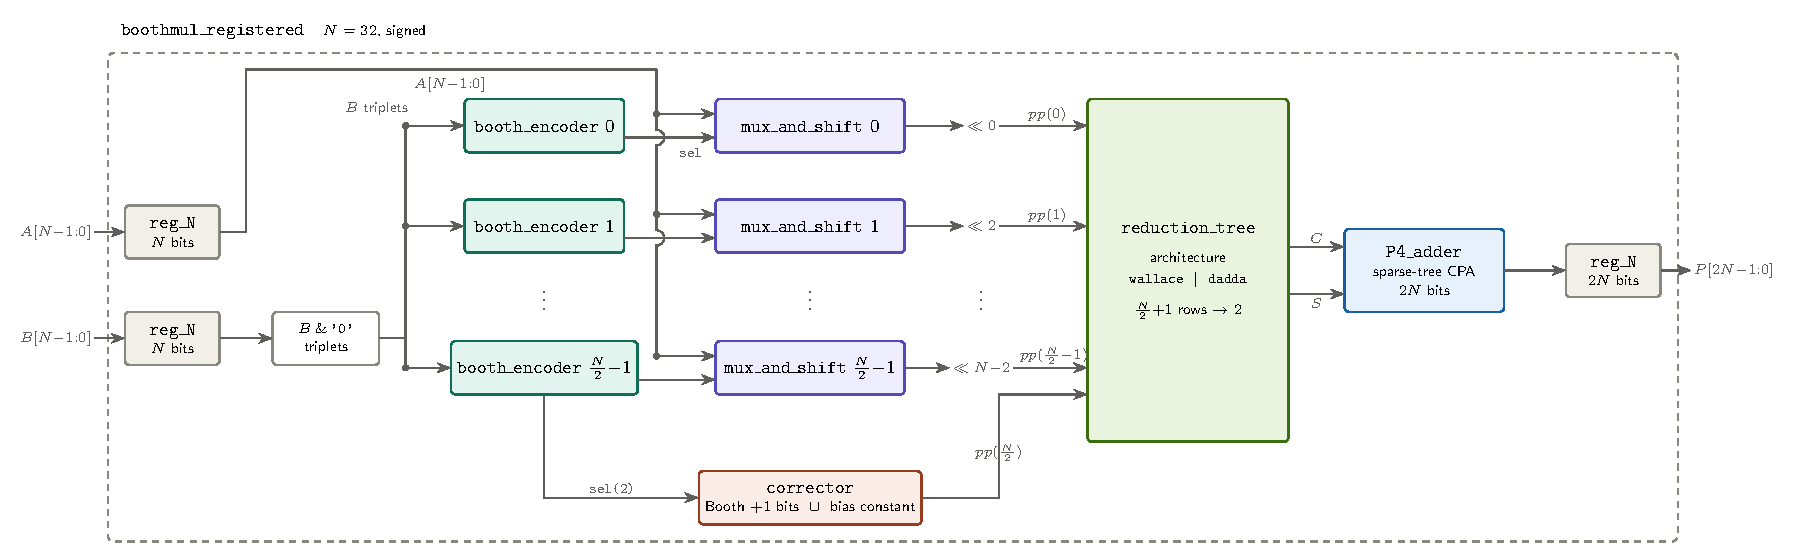
\includegraphics[width=\textwidth]{schematic.pdf}
\caption{Top level of the structural multiplier. The partial-product rows are
drawn generically: there are $N/2$ of them plus the corrector row. Only
\texttt{reduction\_tree} differs between the Wallace and Dadda variants, and
only \texttt{mux\_and\_shift} differs between the sign-extension variants.}
\label{fig:schem}
\end{figure}

\subsection{Radix-4 modified Booth recoding}

A direct implementation of an $N\times N$ product accumulates one shifted copy
of $A$ per bit of $B$, giving $N$ partial-product rows. Radix-4 modified Booth
recoding inspects overlapping triplets of $B$ --- bits
$(2i{+}1,\,2i,\,2i{-}1)$ with the convention $B_{-1}=0$ --- and maps each
triplet to a single signed digit $d_i\in\{0,\pm1,\pm2\}$, so that

\begin{equation}
A \cdot B \;=\; \sum_{i=0}^{N/2-1} d_i \, A \cdot 4^{\,i}.
\label{eq:booth}
\end{equation}

\begin{table}[!ht]
\centering\small
\begin{tabular}{@{}cccl@{}}
\toprule
\textbf{triplet} & \textbf{digit }$d_i$ & \textbf{\texttt{sel}} & \textbf{row generated} \\
\midrule
000,\ 111 & $0$    & 000 & all zeros \\
001,\ 010 & $+1$   & 001 & $+A$  \\
011       & $+2$   & 011 & $+2A$ \\
100       & $-2$   & 111 & $-2A$ \\
101,\ 110 & $-1$   & 101 & $-A$  \\
\bottomrule
\end{tabular}
\caption{Radix-4 modified Booth recoding as implemented in
\texttt{booth\_encoder}. The control vector is
\texttt{sel = \{neg, double, enable\}}.}
\label{tab:booth}
\end{table}

The number of rows is therefore $N/2$ rather than $N$. This halving is the
principal benefit of the recoding, because the reduction tree that follows is
the dominant contributor to both area and delay, and its cost grows with the
number of rows. Multiplication by two is a wired shift and costs nothing.
Negation is not free: it is the origin of two of the three optimizations
presented below.

\subsection{Datapath organisation}

The datapath consists of five stages.

\begin{table}[!ht]
\centering\small
\begin{tabular}{@{}lll@{}}
\toprule
\textbf{Stage} & \textbf{Entity} & \textbf{Function} \\
\midrule
encode    & \texttt{booth\_encoder}  & triplet of $B$ $\rightarrow$ \texttt{sel = \{neg, double, enable\}} \\
generate  & \texttt{mux\_and\_shift} & one partial-product row: $0$, $\pm A$, $\pm 2A$ \\
correct   & \texttt{corrector}       & one additional row: Booth increments and the bias constant \\
reduce    & \texttt{reduction\_tree} & $N/2{+}1$ rows $\rightarrow$ carry and sum vectors \\
add       & \texttt{P4\_adder}       & sparse-tree carry-propagate adder $\rightarrow$ $2N$-bit product \\
\bottomrule
\end{tabular}
\caption{Stages of the structural multiplier. The synthesis top level,
\texttt{boothmul\_registered}, wraps this combinational block between input and
output registers.}
\end{table}

Row $i$ carries weight $4^i$, applied as a left shift of $2i$ positions in
\texttt{boothmul}. The reduction tree is deliberately separated from the final
carry-propagate adder, so that the reduction strategy can be replaced without
touching any other file.

\subsection{Exactness modulo $2^{2N}$}
\label{sec:modular}

Three mechanisms in this design discard information: the carry-save adders drop
the carry generated by the most significant column, the final adder's carry-out
is left unconnected, and the sign-extension optimization of
Section~\ref{sec:opt1} deliberately introduces a bias that is cancelled later.
All three are exact, for the same reason.

The datapath computes in the ring $\mathbb{Z}/2^{2N}\mathbb{Z}$. Every
operation performed on the $2N$-bit vectors --- addition, carry-save addition,
shifting, and the final carry-propagate addition --- is a ring operation, so
discarding any carry out of bit $2N-1$ is a reduction modulo $2^{2N}$ and
commutes with everything that follows. The product of two $N$-bit two's
complement operands lies in $[-2^{2N-2},\,2^{2N-2}]$, which is representable in
$2N$ bits, so its residue class modulo $2^{2N}$ determines it uniquely.

It is therefore sufficient to show that the array of rows delivered to the
reduction tree is congruent to $A\cdot B$ modulo $2^{2N}$. Intermediate values
may overflow freely; only the congruence matters. This property is what makes
the derivation in Section~\ref{sec:opt1} valid, and it is the reason a constant
may be added to the array to cancel a bias without any range analysis.

% =====================================================================
\section{Optimization 1: elimination of the partial-product sign extension}
\label{sec:opt1}

\subsection{Row format and the cost of explicit sign extension}

The term $m_i = d_i A$ generated for row $i$ lies in $[-2^N,\,2^N-2]$ and is
therefore representable in $N+1$ bits of two's complement. It must be placed in
a $2N$-bit array at weight $2^{2i}$. Because $m_i$ is signed and the array is
summed as an unsigned quantity, bit $N$ of the row must be replicated upward
from position $N+2i$ to position $2N-1$.

The number of replicated bits in row $i$ is $N-1-2i$, so across the array

\begin{equation}
\sum_{i=0}^{N/2-1} \bigl(N-1-2i\bigr)
\;=\; \frac{N}{2}(N-1) - \frac{N}{2}\Bigl(\frac{N}{2}-1\Bigr)
\;=\; \frac{N^2}{4}
\label{eq:secost}
\end{equation}

partial-product bits exist only to carry sign information. At $N=32$ this is
$256$ bits out of a total of $800$, close to one third of the array. Each of
them must be generated, routed, and compressed by the reduction tree, and none
carries information beyond the single bit it replicates.

\subsection{The inversion identity}

Let $s$ denote the sign bit of $m_i$, that is $m_{i,N}$. In two's complement,

\begin{equation}
m_i \;=\; -s\cdot 2^N + \sum_{j=0}^{N-1} m_{i,j}\,2^{\,j}.
\end{equation}

Since $s + \bar{s} = 1$ for a single bit, $-s = \bar{s} - 1$, and therefore

\begin{equation}
-s\cdot 2^N \;=\; \bar{s}\cdot 2^N - 2^N.
\label{eq:identity}
\end{equation}

Define the \emph{stored} row as

\begin{equation}
R_i \;=\; \bar{s}\cdot 2^N + \sum_{j=0}^{N-1} m_{i,j}\,2^{\,j},
\end{equation}

that is: the $N$ low bits unchanged, the sign bit inverted, and zeros above.
Substituting \eqref{eq:identity} gives the exact relation

\begin{equation}
m_i \;=\; R_i - 2^N.
\label{eq:rowbias}
\end{equation}

The sign extension has been replaced by a single inverted bit. What remains is
a constant error of exactly $2^N$ per row, independent of $A$, of the Booth
digit, and of the row index. It is not an approximation, and it does not depend
on the data.

\subsection{Closed form of the correction constant}

Applying \eqref{eq:rowbias} to \eqref{eq:booth}, the array of stored rows
overshoots the product by

\begin{equation}
E \;=\; \sum_{i=0}^{N/2-1} 2^{\,N+2i}
     \;=\; 2^N \cdot \frac{4^{N/2}-1}{3}
     \;=\; \frac{2^N\bigl(2^N-1\bigr)}{3}.
\label{eq:E}
\end{equation}

By Section~\ref{sec:modular} the correction is the additive inverse of $E$ in
$\mathbb{Z}/2^{2N}\mathbb{Z}$:

\begin{equation}
C \;=\; 2^{2N} - \frac{2^N\bigl(2^N-1\bigr)}{3}
   \;=\; 2^N\left(2^N - \frac{2^N-1}{3}\right).
\label{eq:C}
\end{equation}

Two properties of \eqref{eq:C} are structurally important. First, $C$ is a
multiple of $2^N$, so its lower $N$ bits are zero. Second, for even $N$ the
quantity $(2^N-1)/3$ has the binary form $0101\ldots01$, and subtracting it from
$2^N$ yields $1010\ldots1011$. The constant therefore occupies bits $2N-1$ down
to $N$ with the hexadecimal pattern $\mathtt{AA}\ldots\mathtt{AB}$.

\begin{table}[!ht]
\centering\small
\begin{tabular}{@{}rrl@{}}
\toprule
$N$ & $E$ & $C$, bits $2N{-}1$ down to $N$ \\
\midrule
 4 & $80$                 & \texttt{0xB} \\
 8 & $21\,760$            & \texttt{0xAB} \\
16 & $1.43\times10^{9}$   & \texttt{0xAAAB} \\
32 & $6.14\times10^{18}$  & \texttt{0xAAAAAAAB} \\
\bottomrule
\end{tabular}
\caption{The correction constant for several operand widths. The repeating
pattern is a direct consequence of the factor $1/3$ in \eqref{eq:E}.}
\label{tab:const}
\end{table}

The constant is generated at elaboration time by \texttt{sign\_ext\_const} in
\texttt{common\_pkg}. It is built bit by bit rather than arithmetically, because
$C$ is a $2N$-bit quantity and the VHDL integer type cannot represent it at
$N=32$:

\begin{lstlisting}[style=vhdl]
function sign_ext_const(NB : natural) return std_logic_vector is
  variable v : std_logic_vector(2*NB-1 downto 0) := (others => '0');
begin
  v(NB) := '1';                      -- the trailing B
  for j in NB+1 to 2*NB-1 loop       -- the repeating A above it
    if (j mod 2) = 1 then v(j) := '1'; end if;
  end loop;
  return v;
end function;
\end{lstlisting}

\subsection{Absorption into the Booth increment row}

Radix-4 Booth already requires one additional row. A negated row is produced as
a one's complement by \texttt{mux\_and\_shift}; the matching $+1$ is not added
locally but collected across all rows, with $\mathtt{sel}(2)$ of row $i$ placed
at weight $2^{2i}$. This increment row occupies only the even positions of the
lower half of the array.

The correction constant $C$ occupies only the upper half. The two therefore
share one row without collision, and the entire cost of Optimization~1 is
confined to the upper half of a row the design already had. The
\texttt{corrector} entity builds it:

\begin{lstlisting}[style=vhdl]
architecture no_sign_extend of corrector is
  constant SE_CONST : std_logic_vector(2*N-1 downto 0) := sign_ext_const(N);
begin
  gen_neg: for i in 0 to N/2-1 generate      -- low half: Booth increments
    correction_v(2*i)   <= neg_bits(i);
    correction_v(2*i+1) <= '0';
  end generate;
  correction_v(2*N-1 downto N) <= SE_CONST(2*N-1 downto N);  -- high half
end architecture;
\end{lstlisting}

The high half is a tie to the supply rails. It contains no logic, and the
synthesis tool propagates it as constants through the first reduction stage.

\subsection{Implementation}

The two row formats are alternative architectures of \texttt{mux\_and\_shift}.
The baseline sign-extends to $2N$ bits; the optimized version constructs the row
in $N+1$ bits, inverts bit $N$, and zero-fills above:

\begin{lstlisting}[style=vhdl]
-- architecture sign_extend
q := std_logic_vector(resize(signed(A), 2*N));     -- full-width row
...
q := q xor (q'range => sel(2));
pp <= q;

-- architecture no_sign_extend
q := std_logic_vector(resize(signed(A), N+1));     -- N+1 bits only
...
q := q xor (q'range => sel(2));
q(N) := not q(N);                                  -- stored sign
pp   <= std_logic_vector(resize(unsigned(q), 2*N));
\end{lstlisting}

The two row formats define two corrector architectures. The
\texttt{no\_sign\_extend} format biases every row by $+2^{\,2i+N}$, which
\texttt{corrector(no\_sign\_extend)} cancels; the baseline format has no bias and
takes \texttt{corrector(sign\_extend)}. Each pair is bound as a unit by the
configurations in \texttt{cfg/}.

\subsection{Measured effect}

The array shrinks from $800$ to $561$ partial-product bits, a reduction of
$29.9\%$. At relaxed timing the synthesised area falls from
$6346\,\mathrm{um}^2$\src{R1} to $5975\,\mathrm{um}^2$\src{R2},
a reduction of $5.8\%$, and the cell count at a $3.0$\,ns constraint falls from
$4639$ to $4455$\src{R7}.

The area reduction is much smaller than the reduction in partial-product bits.
The removed bits are constant-valued sign replications, and constant propagation
in \texttt{compile\_ultra} eliminates most of the associated logic independently
of the optimization. The contribution that constant propagation cannot make is
the reduction in structural column height, which determines the size of the
reduction network; that is what Optimization~2 exploits.

% =====================================================================
\section{Optimization 2: a generic Dadda reduction schedule}
\label{sec:opt2}

The reduction tree is the largest block in the design. This section describes
its replacement by a Dadda schedule computed entirely at elaboration time, for
arbitrary $N$, from the geometry of the partial-product array.

\subsection{Column representation}

The partial-product array is a set of $2N$ columns; column $k$ contains $n_k$
bits, referred to below as \emph{dots}, all of weight $2^k$. A reduction network
compresses every column until no column contains more than two dots, at which
point a carry-propagate adder completes the sum.

The two primitives are the full adder, which takes three dots of column $k$ and
produces one dot in column $k$ (sum) and one in column $k+1$ (carry), and the
half adder, which takes two and produces the same two outputs. A full adder
reduces the total dot count by one; a half adder does not reduce it at all.

This gives an exact invariant, used as a correctness check in
Section~\ref{sec:ddcheck}: if the array begins with $D_0$ dots and terminates
with $D_f$, the number of full adders required is exactly $D_0 - D_f$,
independently of the schedule. Half adders fall outside this accounting: they
occupy cells without contributing to the reduction, so the quality of a schedule
is measured by how few of them it places.

\subsection{Wallace and Dadda placement criteria}

Wallace reduction compresses as early as possible: at every
stage, every group of three dots in a column is given a full adder. Dadda
reduction compresses as late as possible: a target height is fixed
for each stage, and only enough compressors are placed to meet it.

The targets follow the Dadda sequence

\begin{equation}
d_0 = 2, \qquad d_{j+1} = \left\lfloor \tfrac{3}{2}\, d_j \right\rfloor
\quad\Longrightarrow\quad 2,\,3,\,4,\,6,\,9,\,13,\,19,\,28,\ldots
\label{eq:dadda}
\end{equation}

where $d_j$ is the largest column height reducible to two in $j$ stages. The
number of stages needed for $r$ rows is the smallest $j$ with $d_j \geq r$. For
$N=32$ the array has $N/2+1 = 17$ rows, so $d_6 = 19 \geq 17$ and six reduction
stages are required, with targets $13, 9, 6, 4, 3, 2$.

Both quantities are implemented in \texttt{dadda\_types\_pkg}:

\begin{lstlisting}[style=vhdl]
function height_dadda(lev : natural) return natural is
  variable temp : integer := 2;
begin
  for i in 0 to lev-1 loop temp := (temp*3)/2; end loop;
  return temp;
end function;

function num_layers_dadda(NROWS : natural) return natural is
  variable temp : natural := 2;  variable level : natural := 1;
begin
  while NROWS > temp loop
    temp  := height_dadda(level);
    level := level + 1;
  end loop;
  return level;
end function;
\end{lstlisting}

\texttt{NUM\_LAYERS\_D} is declared as a deferred constant in the package
header and given its value in the package body, so that the header can expose it
to the type declarations before \texttt{num\_layers\_dadda} is defined.

The practical difference between the two strategies is the half-adder count. A
Wallace tree places a half adder wherever a column has two spare dots, and each
one costs cells without reducing the dot count. Dadda places a half adder only
when a column is exactly one dot above its target. For $N=32$ the schedule
computed here uses $45$ half adders across the entire array.

\subsection{Generation of the initial array}

The schedule is derived from the geometry of the array, not from its values, so
it can be computed before any signal exists. The function
\texttt{making\_inital\_layer} returns a Boolean occupancy matrix for the
sign-extension-eliminated layout of Section~\ref{sec:opt1}:

\begin{lstlisting}[style=vhdl]
-- rows 0 .. N/2-1 : N+1 significant bits, shifted by 2i
loop_rows: for ro in 0 to (NBIT/2-1) loop
  for col in ro*2 to ro*2+NBIT loop
    rows(ro)(col) := '1';
  end loop;
end loop;

-- row N/2 : the corrector row
for i in 0 to ((NBIT-1)/2) loop                 -- Booth increments, even weights
  rows(last_row)(i*2) := '1';
end loop;
rows(last_row)(NBIT) := '1';                    -- the trailing B of the constant
for i in 0 to ((NBIT-1)/2) loop                 -- the repeating A above it
  rows(last_row)(i*2 + NBIT+1) := '1';
end loop;
\end{lstlisting}

The three parts of the corrector row correspond term by term to the
decomposition of Section~\ref{sec:opt1}: the Booth increments in the low half,
the bit at position $N$, and the alternating pattern above it. The matrix
encodes the optimized layout, so the Dadda architecture is defined for the
sign-extension-eliminated row format only, and is bound with
\texttt{mux\_and\_shift(no\_sign\_extend)} or
\texttt{mux\_and\_shift(fused\_selector)}.

\subsection{The scheduling algorithm}

\texttt{constructing\_dadda} performs the entire schedule at elaboration time
and returns three matrices of identical shape, indexed by
$(\text{layer},\text{row slot},\text{column})$:

\begin{itemize}\itemsep1pt
\item \texttt{FA\_matrix} --- marks the three source slots of every full adder;
\item \texttt{HA\_matrix} --- marks the two source slots of every half adder;
\item \texttt{remaining\_system} --- the dots no compressor consumed, which pass
      unchanged to the next layer.
\end{itemize}

The three are produced in a single pass. A mark-and-clear discipline guarantees
that they stay mutually consistent: when a dot is assigned to a compressor its
position is written into the corresponding matrix and simultaneously cleared
from the working system, so it can neither be assigned twice nor survive into
the set of passed dots.

\begin{lstlisting}[style=vhdl]
loop_setting_FAs: for i in 0 to (fa_id-1) loop
  node_cnt := 0;  roww := 0;
  while node_cnt < 3 loop
    if system(lev)(roww)(col) = '1' then
      node_cnt := node_cnt + 1;
      FA_matrix(lev)(roww)(col) := '1';   -- record the source slot
      system(lev)(roww)(col)    := '0';   -- and consume it
    end if;
    roww := roww + 1;
  end loop;
end loop;
\end{lstlisting}

Layers are processed from the initial layer downward, and columns within a layer
from least to most significant, because the compressor count of a column depends
on the carries produced by the column below it.

\subsection{Carry accounting}

The height test is the subtle part of the algorithm. The target height applies
to layer $\mathrm{lev}-1$, and column $k$ of that layer receives dots from three
distinct sources:

\begin{enumerate}\itemsep1pt
\item $C_{\mathrm{in}}$ carries generated by column $k-1$ of the \emph{same}
      stage, written into layer $\mathrm{lev}-1$ when column $k-1$ was
      processed;
\item one sum bit per compressor placed in column $k$;
\item the dots of column $k$ that no compressor consumed.
\end{enumerate}

If column $k$ holds $n$ dots at layer $\mathrm{lev}$ and is given $F$ full
adders and $H$ half adders, the resulting height at layer $\mathrm{lev}-1$ is

\begin{equation}
C_{\mathrm{in}} + (F+H) + \bigl(n - 3F - 2H\bigr)
\;=\; C_{\mathrm{in}} + n - 2F - H,
\end{equation}

so the compressor count must satisfy
$C_{\mathrm{in}} + n - 2F - H \leq d_{\mathrm{lev}-1}$. A column is therefore
sized against a quantity that does not exist in its own layer. A test that
counts only the dots of column $k$ satisfies the target locally but not
globally: columns exceed their target height and the array does not reach two
rows within the allotted number of stages.

The loop implements exactly this, using the fact that a full adder removes two
dots from the height and a half adder removes one:

\begin{lstlisting}[style=vhdl]
count_temp := count + C_out_count;     -- own dots plus carries from col-1
while (count_temp > max_height) loop
  if    count_temp >= (max_height + 2) then
    count_temp := count_temp - 2;  fa_id := fa_id + 1;
  elsif count_temp  = (max_height + 1) then
    ha_flag := 1;  count_temp := count_temp - 1;
  end if;
end loop;
\end{lstlisting}

The half-adder branch is reached only when the residual excess is exactly one,
which is the property that keeps the half-adder count low.

\subsection{Slot allocation}

A compressor instantiated in the netlist must know which row slot of the next
layer its outputs drive. The allocation order for column $k$ of layer
$\mathrm{lev}-1$ is fixed:

\begin{center}\small
\begin{tabular}{@{}ll@{}}
\toprule
slots $0 \ldots C_{\mathrm{in}}-1$ & carries arriving from column $k-1$ \\
slots $C_{\mathrm{in}} \ldots C_{\mathrm{in}}+F+H-1$ & sums of this column's compressors \\
remaining slots & dots passed through unchanged \\
\bottomrule
\end{tabular}
\end{center}

This order must be reproduced identically in two places: in
\texttt{constructing\_dadda}, which writes the matrices, and in
\texttt{dadda\_tree}, which writes the port maps. The difficulty is that a
\texttt{generate} statement carries no sequential state --- each instance is
elaborated independently and cannot inherit a running counter from the previous
column --- so every offset must be recomputable from the matrices alone. This is
the purpose of the analysis functions in \texttt{dadda\_math\_pkg}.

\begin{table}[!ht]
\centering\small
\begin{tabular}{@{}ll@{}}
\toprule
\textbf{Function} & \textbf{Returns} \\
\midrule
\texttt{num\_rows\_dadda(lev)}                & occupied row slots at layer \texttt{lev} \\
\texttt{fa\_count\_col\_dadda(\ldots)}        & number of full adders in a column \\
\texttt{ha\_flag\_col\_dadda(\ldots)}         & $1$ if the column has a half adder, else $0$ \\
\texttt{num\_C\_out\_from\_prev\_col(\ldots)} & $C_{\mathrm{in}}$, recomputed from column $k-1$ \\
\texttt{fa\_arg\_func(\ldots)}                & the three source row indices of each full adder \\
\texttt{ha\_arg\_func(\ldots)}                & the two source row indices of the half adder \\
\texttt{remaining\_counting\_func(\ldots)}    & number of passed dots in a column \\
\texttt{remaining\_bit\_pos(\ldots)}          & their row indices \\
\bottomrule
\end{tabular}
\caption{Analysis functions used to recover port-map positions from the
scheduling matrices. All are pure and evaluated at elaboration time.}
\label{tab:helpers}
\end{table}

\texttt{num\_C\_out\_from\_prev\_col} resolves the generate-statement constraint
directly: instead of propagating $C_{\mathrm{in}}$ forward, it recomputes it by
counting the compressors of column $k-1$ in the same layer. Two assertions
enforce the schedule invariants at elaboration time --- at most one half adder
per column, and unique half-adder source positions --- so that a violation
terminates elaboration rather than producing a mis-wired tree.

The structural instantiation then reads directly from the matrices. The generate
nest is three levels deep --- layer, column, compressor --- and its constant
declarations carry all the positional information:

\begin{lstlisting}[style=vhdl]
columns: for col in 0 to NBIT*2-1 generate
  constant fa_count_col   : integer := fa_count_col_dadda(FA_matrix, lev, num_rows_current, col);
  constant C_out_counting : integer := num_C_out_from_prev_col(FA_matrix, HA_matrix, lev, col);
  constant FA_args        : fa_args_t(0 to fa_count_col-1)
                          := fa_arg_func(FA_matrix, num_rows_current, fa_count_col, lev, col);
begin
  maping_fa: for ID in 0 to fa_count_col-1 generate
    constant sum_bit_arg   : integer := ID + C_out_counting;
    constant carry_out_arg : integer := ID;
  begin
    FA_i : FA port map (
      A  => layer(lev)(FA_args(ID)(0))(col),
      B  => layer(lev)(FA_args(ID)(1))(col),
      Ci => layer(lev)(FA_args(ID)(2))(col),
      S  => layer(lev-1)(sum_bit_arg)(col),
      Co => layer(lev-1)(carry_out_arg)(col+1));
  end generate;
\end{lstlisting}

\subsection{Consistency and generic cost}
\label{sec:ddcheck}

The schedule was validated against the dot-count invariant. For the optimized
layout at $N=32$ the array begins with $D_0 = 561$ dots and terminates with
$D_f = 126$, so exactly $561 - 126 = 435$ full adders are necessary; the
schedule produces $435$. The identity holds at every width tested, and row $2$
of the final layer is empty at all widths, confirming that the reduction really
does terminate at two rows.

\begin{table}[!ht]
\centering\small
\begin{tabular}{@{}rrrrrrrrr@{}}
\toprule
& & \multicolumn{2}{c}{\textbf{array dots}} & \multicolumn{4}{c}{\textbf{Dadda}} & \textbf{Wallace} \\
\cmidrule(lr){3-4}\cmidrule(lr){5-8}\cmidrule(lr){9-9}
$N$ & rows & baseline & optimized & stages & FA & HA & cells & FA instances \\
\midrule
 8 &  5 &   56 &   45 & 3 &   15 &  9 &   24 &   48 \\
16 &  9 &  208 &  153 & 4 &   91 & 21 &  112 &  224 \\
32 & 17 &  800 &  561 & 6 &  435 & 45 &  480 &  960 \\
64 & 33 & 3136 & 2145 & 8 & 1891 & 93 & 1984 & 3968 \\
\bottomrule
\end{tabular}
\caption{Cost of the reduction network as a function of operand width, computed
from the elaboration-time schedule. The Wallace column gives the number of full
adder instances written by the row-wise implementation: $2N$ per carry-save
adder, with no allowance for columns that are not full.}
\label{tab:generic}
\end{table}

Table~\ref{tab:generic} quantifies the structural difference. The Wallace
implementation instantiates carry-save adders across the full $2N$ width, giving
$960$ full adder instances at $N=32$ against $435$ full adders and $45$ half
adders for Dadda. Many of the Wallace instances have constant inputs and are
removed by the synthesis tool, so the difference in the synthesised result is
smaller than the ratio suggests. It is not zero, because constant propagation
cannot recover the shorter critical path that a column-scheduled tree provides.

\subsection{Constraints imposed by VHDL-93}

Three language restrictions shaped the implementation.

\paragraph{Generate bounds must be globally static.} The number of compressors
in a column is data of the schedule, so the schedule must be available as a
constant expression before elaboration of the generate statement. This is why it
is computed by a pure function over Boolean matrices rather than derived
incrementally while the structure is built.

\paragraph{A package cannot see a generic.} The port type \texttt{pp\_array}
must be declared in a package so that both the entity and its instantiators can
see it, and a VHDL-93 package has no visibility of generics. The operand width
is therefore a constant, \texttt{NBIT} in \texttt{common\_pkg}, rather than a
generic of the top-level entity. The design remains generic in the sense that
every downstream quantity is a function of \texttt{NBIT}; changing that one
constant reconfigures the multiplier, the reduction schedule and the testbench
together.

\paragraph{Deferred constants.} \texttt{NUM\_LAYERS\_D} is required by the type
declarations in the package header but computed by a function defined in the
package body. It is declared without a value in the header and given one in the
body.

\subsection{Measured effect}

At relaxed timing the area falls from $5975\,\mathrm{um}^2$\src{R2} to
$5620\,\mathrm{um}^2$\src{R3}, a further $5.9\%$, and the minimum
achieved period improves from $1.87$\,ns to $1.78$\,ns\src{R3} --- the largest
single improvement in delay among the three optimizations. The cell count at a
$3.0$\,ns constraint falls from $4455$ to $3936$\src{R7}.

% =====================================================================
\section{Optimization 3: fusion of the Booth selector}
\label{sec:opt3}

\subsection{Cost of the separate negation stage}

After Optimization~2 the design is $1180\,\mathrm{um}^2$ larger than the
inferred reference. A cell census of the two netlists at a $3.0$\,ns
constraint\src{R7} localises the difference.

\begin{table}[!ht]
\centering\small
\begin{tabular}{@{}lrrrr@{}}
\toprule
& \textbf{XOR + XNOR} & \textbf{FA cells} & \textbf{INV} & \textbf{total cells} \\
\midrule
Structural, Dadda            & 1230 & 117 & 505 & 3936 \\
Inferred \texttt{A * B}      &  559 & 268 & 311 & 3035 \\
\bottomrule
\end{tabular}
\caption{Cell census at a $3.0$\,ns constraint\src{R7}, before Optimization~3.}
\end{table}

The structural design contains $671$ more exclusive-or cells than the inferred
one, and maps only $117$ of its $435$ scheduled full adders to library adder
cells. Both follow from the structure of \texttt{mux\_and\_shift}, which builds
a row in two steps: a multiplexer selects $A$, $2A$ or zero, and every bit of
the result is then exclusive-ored with $\mathtt{sel}(2)$ to perform the
negation. That is $N+1$ XOR2 cells per row across $16$ rows, or $528$ cells at
$N=32$, approximately $843\,\mathrm{um}^2$ performing nothing but
conditional inversion.

The indirect cost is the larger of the two. A full adder is itself an
exclusive-or-dominated function. With a layer of XOR gates immediately feeding
the reduction tree, the logic cones presented to the technology mapper mix
negation and compression, and the mapper decomposes them into generic gates
rather than matching the \texttt{FA\_X1} pattern. The low adder-cell count is
therefore a consequence of the XOR layer and not an independent effect.

\subsection{Algebraic formulation}

The multiplexer and the conditional inversion can be merged into one function.
Let

\begin{align}
\mathrm{src}_1 &= A_{N-1} \,\Vert\, A            &&\text{($A$ in $N+1$ bits)}\\
\mathrm{src}_2 &= A \,\Vert\, \mathtt{'0'}       &&\text{($2A$ in $N+1$ bits)}
\end{align}

and decode the control vector once per row into four mutually exclusive
conditions:

\begin{equation}
\begin{aligned}
c_{+1} &= \mathtt{sel}(0)\cdot\overline{\mathtt{sel}(1)}\cdot\overline{\mathtt{sel}(2)}, &\qquad
c_{-1} &= \mathtt{sel}(0)\cdot\overline{\mathtt{sel}(1)}\cdot\mathtt{sel}(2), \\
c_{+2} &= \mathtt{sel}(0)\cdot\mathtt{sel}(1)\cdot\overline{\mathtt{sel}(2)}, &\qquad
c_{-2} &= \mathtt{sel}(0)\cdot\mathtt{sel}(1)\cdot\mathtt{sel}(2).
\end{aligned}
\end{equation}

Each output bit is then a four-term sum of products:

\begin{equation}
q_i \;=\; c_{+1}\,\mathrm{src}_{1,i}
     \;+\; c_{-1}\,\overline{\mathrm{src}_{1,i}}
     \;+\; c_{+2}\,\mathrm{src}_{2,i}
     \;+\; c_{-2}\,\overline{\mathrm{src}_{2,i}},
\label{eq:fused}
\end{equation}

after which sign-extension elimination is applied exactly as before:
$pp_N = \overline{q_N}$, $pp_{N-1:0} = q_{N-1:0}$, and zeros above.

\subsection{Completeness of the cover}

Equation~\eqref{eq:fused} enumerates four of the five possible row values; the
zero row is covered implicitly, because all four conditions are false when
$\mathtt{sel}(0)=0$ and the sum of products evaluates to zero. The cover is
complete provided the encoder never asserts $\mathtt{sel}(2)$ with
$\mathtt{sel}(0)$ deasserted --- that is, never requests a negated zero row.
Table~\ref{tab:booth} confirms this: the only codes with $\mathtt{sel}(2)=1$ are
$101$ and $111$, both of which have $\mathtt{sel}(0)=1$. The property follows
from the encoding table and is not an assumption imposed on it.

\subsection{Effect on technology mapping}

Equation~\eqref{eq:fused} is a two-level sum of products over four literals, and
the Nangate library provides compound AND-OR-invert cells that implement it in a
single stage. No exclusive-or appears anywhere in the row generator. The
complemented terms $\overline{\mathrm{src}_1}$ and $\overline{\mathrm{src}_2}$
are the same function of $A$ in all $N/2$ rows, so common-subexpression
elimination shares one set of inverters across the array.

\begin{table}[!ht]
\centering\small
\begin{tabular}{@{}lrrrrr@{}}
\toprule
& \textbf{XOR + XNOR} & \textbf{FA cells} & \textbf{AOI/OAI} & \textbf{total cells} & \textbf{area} \\
\midrule
Dadda, separate negation & 1230 & 117 & 1405 & 3936 & 5725\,um$^2$ \\
Dadda, fused selector    &   85 & 448 & 1311 & 2819 & 5125\,um$^2$ \\
Inferred \texttt{A * B}  &  559 & 268 &  950 & 3035 & 4910\,um$^2$ \\
\bottomrule
\end{tabular}
\caption{Cell census at a $3.0$\,ns constraint\src{R7}. The adder-cell count
rises from $117$ to $448$, close to the $435$ full adders and $45$ half adders
the schedule specifies.}
\label{tab:census3}
\end{table}

Exclusive-or cells fall from $1230$ to $85$, and the adder-cell count rises from
$117$ to $448$, within $7\%$ of the $480$ compressors the schedule contains.
With the XOR layer removed, the mapper matches the compressors already present
in the RTL. This is why a rewrite confined to a single architecture produces the
largest area reduction of the three optimizations.

\subsection{Measured effect}

Area falls from $5620\,\mathrm{um}^2$\src{R3} to
$5029\,\mathrm{um}^2$\src{R4}, a reduction of $10.5\%$, and the minimum
achieved period improves from $1.78$\,ns to $1.76$\,ns\src{R4}. Total cell count
falls by $28\%$.

% =====================================================================
\section{Functional verification}
\label{sec:verif}

All variants share one self-checking testbench, \texttt{tb\_multiplier}, which
reads the operand width from \texttt{common\_pkg} and selects its coverage mode
accordingly.

\begin{table}[!ht]
\centering\small
\begin{tabular}{@{}ll@{}}
\toprule
\texttt{NBIT} & coverage \\
\midrule
$\leq 8$ & exhaustive --- all $2^{2N}$ operand pairs ($65\,536$ at $N=8$) \\
$> 8$    & corner cases $\{0, \pm1, 2^{N-1}-1, -2^{N-1}\}$ plus $20\,000$ random pairs \\
\bottomrule
\end{tabular}
\end{table}

The reference model is \texttt{signed(A) * signed(B)} truncated to $2N$ bits,
evaluated independently of the design. Mismatches are counted rather than
asserted, so a failing variant reports the number of failing vectors.

Every variant is verified exhaustively at $N=8$ before being synthesised at
$N=32$. Exhaustive coverage at the smaller width is stronger evidence than
random coverage at the larger one, because the properties under test --- the
recoding table, the bias cancellation of Section~\ref{sec:opt1}, the
completeness of the four-term cover of Section~\ref{sec:opt3}, and the column
schedule of Section~\ref{sec:opt2} --- are structural. Each is a statement about
the construction of the array rather than about particular operand values, and
each fails identically at both widths.

Each synthesis configuration has a matching testbench configuration
(Appendix~\ref{app:code}), so the binding verified in simulation is the binding
that is synthesised.

% =====================================================================
\section{Synthesis methodology}
\label{sec:method}

\subsection{Flow and constraints}

The synthesis top level is \texttt{boothmul\_registered}, which places the
combinational multiplier between input and output registers. This makes the
critical path internal --- register to register through the multiplier --- so
that the reported timing measures the design rather than the test environment.

\begin{table}[!ht]
\centering\small
\begin{tabular}{@{}ll@{}}
\toprule
Library            & \texttt{NangateOpenCellLibrary}, typical ECSM \\
Tool               & Synopsys Design Compiler W-2024.09-SP2, \texttt{compile\_ultra} \\
Wire load model    & \texttt{5K\_hvratio\_1\_4} \\
Clock              & \texttt{create\_clock -period \$clockPeriod}, swept \\
Clock uncertainty  & $0.05$\,ns; transition $0.05$\,ns; latency $0.05$\,ns \\
Input delay        & $0.25$\,ns, absolute \\
Output delay       & $0.15$\,ns, absolute \\
Driving cell       & \texttt{BUF\_X4}; output load $0.05$\,pF \\
Max transition     & $0.20$\,ns \\
Area constraint    & \texttt{set\_max\_area 0} \\
Sweep              & $21$ periods from $1.0$ to $6.0$\,ns, $6$ configurations \\
\bottomrule
\end{tabular}
\caption{Synthesis environment. The same constraint file is sourced once per
period; \texttt{\$clockPeriod} is the only quantity that changes.}
\label{tab:env}
\end{table}

The input and output delays are absolute values rather than fractions of the
clock period. This is deliberate and is a precondition for the metric defined in
Section~\ref{sec:achieved}: if the port constraints scaled with the period, the
slack reported at one period could not be compared with the slack reported at
another. Because the design is registered on both sides, the port paths
terminate at a flip-flop within a few gates and never become critical, even at
the tightest constraint. The timing reports confirm this: the critical path runs
from a bit of the $B$ register to the most significant bit of the product
register in every run of the sweep.

The clock and reset networks are marked \texttt{set\_dont\_touch\_network} and
\texttt{set\_ideal\_network}, since clock tree construction belongs to
place-and-route and not to this flow.

\subsection{The achieved period metric}
\label{sec:achieved}

A synthesis run that fails to meet its constraint still produces a valid
netlist, slower than requested. Discarding such runs would discard the fastest
netlists in the sweep, because the tool produces its most aggressive structures
only under a constraint tight enough to force them.

The quantity reported here is therefore the period the netlist actually
supports:

\begin{equation}
T_{\mathrm{achieved}} \;=\; T_{\mathrm{constraint}} - \mathrm{slack}.
\label{eq:achieved}
\end{equation}

Slack is negative for a violated path, so a violated run yields
$T_{\mathrm{achieved}} > T_{\mathrm{constraint}}$. The identity is exact only
when every timing quantity other than the clock is independent of
$T_{\mathrm{constraint}}$, which is why the port delays in Table~\ref{tab:env}
are absolute; clock uncertainty, transition and latency are likewise fixed.

As an example, the fused-selector variant constrained at $1.0$\,ns reports a
slack of $-0.76$\,ns\src{R4}, so the netlist supports $1.76$\,ns. No run in the
sweep produced a faster netlist for that variant, and the tightest constraint
gave the fastest netlist for every variant, which indicates that the left edge of
the achievable region has not been reached at $1.0$\,ns.

\subsection{Non-monotonicity of the optimizer}

Area is not a monotonic function of the clock constraint under
\texttt{compile\_ultra}. Relaxing the period can produce a larger netlist: for
the Wallace baseline the run at $1.1$\,ns is larger than the run at
$1.0$\,ns\src{R1}, and similar reversals occur elsewhere in the sweep.

The behaviour is not attributable to the area constraint. A controlled sweep
with \texttt{set\_max\_area 0} removed\src{R8} gives identical minimum achieved
periods, area differences below $3\%$, and the same non-monotonicity. The cause
is the heuristic nature of the optimizer.

All curves in Section~\ref{sec:results} are therefore Pareto fronts computed
over the whole sweep rather than raw per-constraint traces: a point is plotted
only if no other run of the same variant is both faster and smaller. Dominated
points are omitted.

% =====================================================================
\section{Results}
\label{sec:results}

\subsection{Area and delay}

\begin{table}[!ht]
\centering\small
\begin{tabular}{@{}lrrrr@{}}
\toprule
\textbf{Variant} & \textbf{min. achieved} & \textbf{min. area} & \textbf{gap closed} & \textbf{ref.} \\
\midrule
Wallace, sign-extended (baseline)  & 1.86\,ns & 6346\,um$^2$ & ---     & \src{R1} \\
\quad $+$ sign-extension elimination & 1.87\,ns & 5975\,um$^2$ & 19.5\% & \src{R2} \\
\quad $+$ Dadda reduction            & 1.78\,ns & 5620\,um$^2$ & 38.1\% & \src{R3} \\
\quad \textbf{$+$ fused selector}    & \textbf{1.76\,ns} & \textbf{5029\,um$^2$} & \textbf{69.1\%} & \src{R4} \\
\midrule
Behavioural Booth (adder chain)    & 2.01\,ns & 6210\,um$^2$ &  7.1\% & \src{R5} \\
Inferred \texttt{A * B}            & 1.63\,ns & 4441\,um$^2$ & reference & \src{R6} \\
\bottomrule
\end{tabular}
\caption{Summary of the sweep. Periods are achieved values per
\eqref{eq:achieved}; areas are the minimum over all constraints.
\emph{Gap closed} is the fraction of the area difference between the baseline
and the inferred reference that the variant recovers.}
\label{tab:summary}
\end{table}

Table~\ref{tab:summary} gives the extremes of each variant. The three
optimizations together recover $69.1\%$ of the area difference between the
structural baseline and the inferred reference, and reduce the delay difference
from $0.23$\,ns to $0.13$\,ns.

The behavioural Booth variant, which replaces the reduction tree with a chain of
signed additions, is the slowest design in the sweep at $2.01$\,ns\src{R5}. It
is nevertheless smaller than the Wallace baseline at relaxed timing, because the
synthesis tool implements the adder chain with its own carry-save structures
rather than the explicitly instantiated ones. It measures what inference
achieves from a structurally poor description; its timing result is the more
informative of its two figures.

\begin{figure}[!ht]
\centering
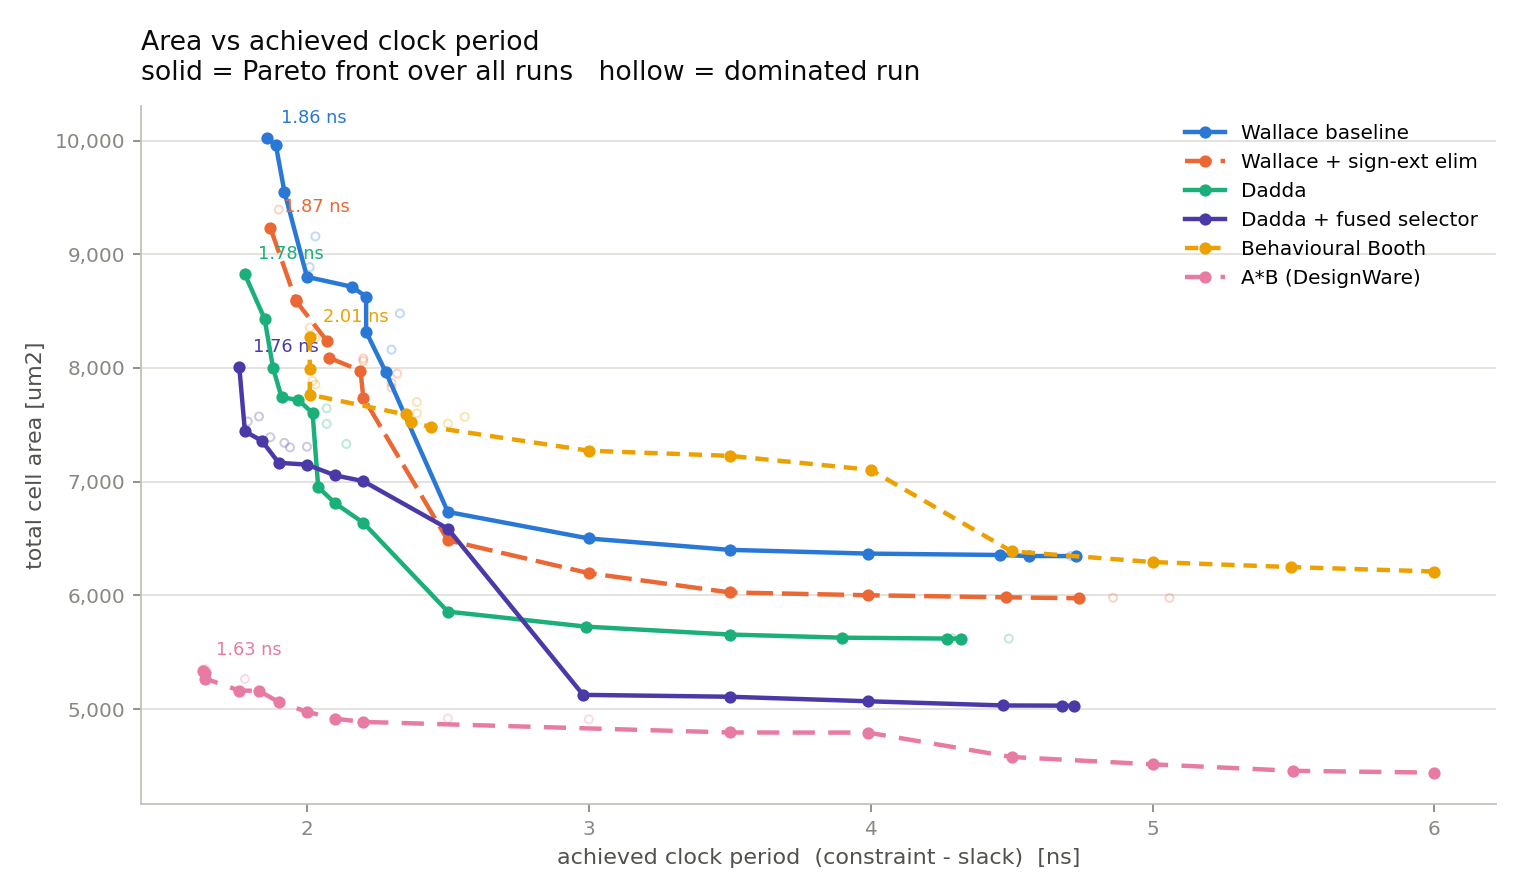
\includegraphics[width=0.94\textwidth]{figures/pareto_area_vs_achieved_main.png}
\caption{Area against achieved period. Each curve is the Pareto front of one
variant over the whole $21$-point sweep; dominated runs are omitted. Lower and
further left is better.}
\label{fig:pareto}
\end{figure}

Figure~\ref{fig:pareto} shows the full fronts. The ordering of the three
optimizations is consistent across the range of periods: each variant dominates
its predecessor almost everywhere, and the separation is largest at relaxed
timing, where the optimizer is free to minimise area rather than spending cells
on speed.

\subsection{Cell-level analysis}

Table~\ref{tab:census3} gives the cell census at a fixed $3.0$\,ns constraint.
Two properties of the sequence follow from it.

The area reduction from Optimization~1 ($5.8\%$) is much smaller than its
reduction in partial-product bits ($29.9\%$), because constant propagation
removes most of the logic associated with sign replication independently of the
optimization. Its contribution is the reduction in structural column height,
which is realised by Optimization~2.

The three optimizations are not independent. The gain of Optimization~3 depends
on Optimization~2, because the compressors the mapper matches after the XOR
layer is removed are the ones the Dadda schedule instantiates. Measured in
isolation, each optimization is smaller than it is in sequence.

\subsection{Crossover in the mid-period region}

\begin{figure}[!ht]
\centering
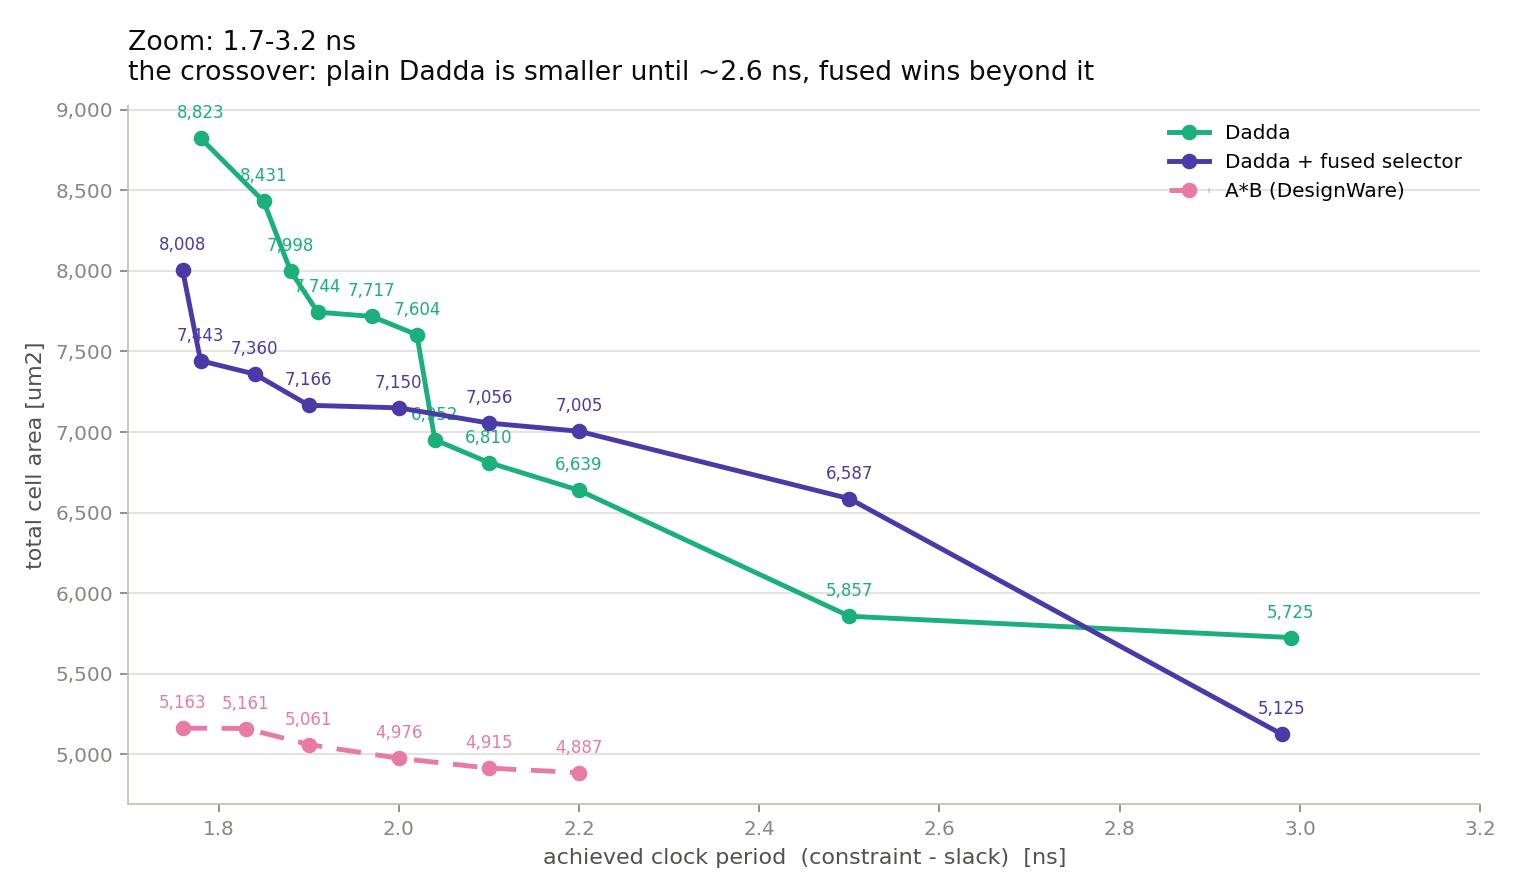
\includegraphics[width=0.84\textwidth]{figures/pareto_zoom_main.png}
\caption{Detail of the region between $1.7$ and $3.1$\,ns. The two Dadda
variants cross twice; near $2.0$\,ns the variant with separate negation is the
smaller of the two.}
\label{fig:zoom}
\end{figure}

The two Dadda variants are not ordered uniformly. Figure~\ref{fig:zoom} shows
that they cross twice, and that near $2.0$\,ns the variant with separate
negation is the smaller of the two. The fused selector presents deeper compound
gates to the optimizer; at intermediate constraints the tool must upsize them to
meet timing, and the upsizing costs more than the exclusive-or cells that were
removed. At relaxed constraints the upsizing is unnecessary and the fused
variant is smaller by $591\,\mathrm{um}^2$; at tight constraints it is
faster.

The crossing is reproduced across adjacent constraint points and appears in the
cell census as a shift in drive strengths rather than in cell counts, which
identifies it as an architectural trade-off rather than run-to-run variation in
the optimizer.

% =====================================================================
\section{Conclusions}

A signed $32\times32$ radix-4 Booth multiplier was implemented in structural
VHDL and optimized in three stages. Measured against an unoptimized Wallace
baseline and an inferred \texttt{A * B} reference synthesised under identical
conditions, the result is a minimum achieved period of $1.76$\,ns against
$1.63$\,ns for the reference, and a minimum area of
$5029\,\mathrm{um}^2$ against $4441\,\mathrm{um}^2$, recovering
$69.1\%$ of the initial area difference.

The three contributions are unequal, and their sizes do not follow the size of
the structural change each one makes. Sign-extension elimination removes
$29.9\%$ of the partial-product bits but only $5.8\%$ of the area, because
constant propagation removes most of the associated logic independently of it.
The Dadda schedule contributes a comparable area reduction and the largest
single improvement in delay, consistent with a shorter and more uniform
reduction depth. Fusing the Booth selector contributes the largest area
reduction of the three, and does so indirectly: its measurable effect is not the
$528$ exclusive-or cells it removes but the $331$ additional full adders the
technology mapper matches once they are gone.

The general result is that the cost of an RTL construct is determined as much by
what it prevents the synthesis tool from matching as by the gates it directly
implies. A single layer of exclusive-or gates between the row generators and the
reduction tree accounts for approximately $600\,\mathrm{um}^2$, most of
it in the logic behind the layer rather than in the layer itself.

Three directions remain open: switching-activity-based power analysis, in which
the removal of $1145$ exclusive-or cells should be more visible than it is in
area; gate-level simulation of each netlist against its SDF; and extension of
the sweep below $1.0$\,ns, since every variant reaches its fastest netlist at
the tightest constraint in the present sweep.

% =====================================================================
\appendix

\section{Source organisation and variant selection}
\label{app:code}

\subsection{Directory layout}

\begin{table}[!ht]
\centering\small
\begin{tabular}{@{}ll@{}}
\toprule
\textbf{Path} & \textbf{Contents} \\
\midrule
\texttt{rtl/common/}              & \texttt{iv}, \texttt{nd2}, \texttt{mux21}, \texttt{mux21\_generic}, \texttt{fa}, \texttt{ha} \\
\texttt{rtl/adder/}               & the P4 sparse-tree carry-propagate adder chain \\
\texttt{rtl/multiplier/}          & encoder, row generator, corrector, CSA, both trees, top levels \\
\texttt{rtl/multiplier/packages/} & the four elaboration-time packages \\
\texttt{tb/}                      & self-checking RTL and gate-level testbenches \\
\texttt{cfg/}                     & design, testbench and synthesis configurations \\
\texttt{sim/}                     & \texttt{compile.do}, \texttt{sim.do} \\
\texttt{synthesis/syn/}           & \texttt{synthesis.tcl}, the SDC, and the report tree \\
\texttt{synthesis/plot\_pareto.py} & reads the reports and produces the figures and tables \\
\bottomrule
\end{tabular}
\end{table}

\subsection{The packages}

\begin{table}[!ht]
\centering\small
\begin{tabular}{@{}ll@{}}
\toprule
\textbf{Package} & \textbf{Contents} \\
\midrule
\texttt{common\_pkg}        & \texttt{NBIT}, \texttt{NROWS}, \texttt{pp\_word}, \texttt{pp\_array}, \texttt{sign\_ext\_const} \\
\texttt{wallace\_math\_pkg} & row counts and layer depth for the uniform carry-save tree \\
\texttt{dadda\_types\_pkg}  & the Dadda height sequence, the matrix types, \texttt{NUM\_LAYERS\_D} \\
\texttt{dadda\_math\_pkg}   & the scheduling function and the port-map analysis functions \\
\bottomrule
\end{tabular}
\end{table}

\texttt{NBIT} is the single width parameter of the project. The design, the
reduction schedule and the testbench all derive from it, so one edit
reconfigures all three consistently.

\subsection{Variant selection}

Each variant is a distinct architecture bound by a configuration. Instances
inside a \texttt{generate} statement require a nested block configuration:

\begin{lstlisting}[style=vhdl]
configuration CFG_BOOTHMUL_DADDA_FUSED_SEL of BOOTHMUL is
  for STRUCTURAL
    for gen_stages                      -- mux_i is inside a generate,
      for mux_i : mux_and_shift         -- hence the nested block configuration
        use entity work.mux_and_shift(fused_selector);
      end for;
    end for;
    for corr_i : corrector
      use entity work.corrector(no_sign_extend);
    end for;
    for tree_i : REDUCTION_TREE
      use entity work.REDUCTION_TREE(dadda);
    end for;
  end for;
end configuration;
\end{lstlisting}

A configuration of \texttt{BOOTHMUL} has no effect on its own, because the
testbench instantiates a \emph{component}. In the absence of a second,
testbench-level configuration, the default binding rule selects the most
recently analysed architecture. Each design configuration therefore has a
matching
\texttt{cfg\_tb\_*} in \texttt{cfg/configurations\_tb.vhd} and a matching
\texttt{CFG\_BOOTHMUL\_REG\_*} in \texttt{cfg/configurations\_synthesis.vhd},
so that the binding simulated is the binding synthesised.

\begin{table}[!ht]
\centering\footnotesize
\begin{tabular}{@{}p{0.60\textwidth}l@{}}
\toprule
\textbf{Binding} & \textbf{Effect} \\
\midrule
\texttt{mux\_and\_shift(sign\_extend)} $+$ \texttt{corrector(sign\_extend)} & baseline \\
\texttt{mux\_and\_shift(no\_sign\_extend)} $+$ \texttt{corrector(no\_sign\_extend)} & Optimization~1 \\
\texttt{mux\_and\_shift(fused\_selector)} $+$ \texttt{corrector(no\_sign\_extend)} & Optimizations~1 and~3 \\
\texttt{reduction\_tree(wallace)} / \texttt{reduction\_tree(dadda)} & Optimization~2 \\
\texttt{mux\_and\_shift(behavioural)} & adder chain \\
\texttt{super\_beh\_multiplier\_registered} & inferred \texttt{A * B} \\
\bottomrule
\end{tabular}
\end{table}

\section{Provenance of the reported measurements}
\label{app:prov}

All measurements are read from the reports in
\texttt{synthesis/syn/reports/}, one directory per configuration and one file
per clock period. File names follow the pattern

\begin{center}
\texttt{<report>\_<CONFIG>\_<period>.rpt}
\end{center}

\noindent
where the period is written with \texttt{p} in place of the decimal point.

\begin{table}[!ht]
\centering\small
\begin{tabular}{@{}lll@{}}
\toprule
\textbf{Tag} & \textbf{Configuration directory} & \textbf{Variant} \\
\midrule
\src{R1} & \texttt{CFG\_BOOTHMUL\_REG\_WAL\_BASE}         & Wallace, sign-extended \\
\src{R2} & \texttt{CFG\_BOOTHMUL\_REG\_WAL\_OPT}          & Wallace, sign extension eliminated \\
\src{R3} & \texttt{CFG\_BOOTHMUL\_REG\_DADDA}             & Dadda, separate negation \\
\src{R4} & \texttt{CFG\_BOOTHMUL\_REG\_DADDA\_FUSED\_SEL} & Dadda, fused selector \\
\src{R5} & \texttt{CFG\_BOOTHMUL\_REG\_BEH}               & behavioural Booth, adder chain \\
\src{R6} & \texttt{CFG\_REG\_SUPER\_BEH}                  & inferred \texttt{A * B} \\
\src{R7} & all of the above, period \texttt{3p0}          & cell census \\
\src{R8} & \texttt{reports\_no\_area\_constraint/}        & controlled run without \texttt{set\_max\_area} \\
\bottomrule
\end{tabular}
\end{table}

\begin{table}[!ht]
\centering\small
\begin{tabular}{@{}lll@{}}
\toprule
\textbf{Quantity} & \textbf{File} & \textbf{Field} \\
\midrule
Area                & \texttt{area\_*.rpt}      & \texttt{Total cell area} \\
Cell counts         & \texttt{reference\_*.rpt} & \texttt{Count} column, summed by cell family \\
Slack               & \texttt{timing\_*.rpt}    & \texttt{slack (MET | VIOLATED)} \\
Critical path ends  & \texttt{timing\_*.rpt}    & \texttt{Startpoint}, \texttt{Endpoint} \\
Achieved period     & derived                   & \eqref{eq:achieved} \\
\bottomrule
\end{tabular}
\end{table}

Structural quantities --- partial-product bit counts, compressor counts and the
stage schedule --- are not read from reports. They are computed from the
elaboration-time functions in \texttt{dadda\_math\_pkg} and
\texttt{wallace\_math\_pkg}, and were cross-checked against the dot-count
invariant of Section~\ref{sec:ddcheck}.

The figures and the summary table are regenerated by

\begin{lstlisting}
cd synthesis
python3 plot_pareto.py syn/reports -o ../docs/figures --zoom 1.7 3.1
\end{lstlisting}

which parses the report tree directly, with no intermediate data file.


\end{document}
